% Created 2016-01-08 Fri 17:04
\documentclass[bigger]{beamer}
\usepackage[utf8]{inputenc}
\usepackage[T1]{fontenc}
\usepackage{fixltx2e}
\usepackage{graphicx}
\usepackage{grffile}
\usepackage{longtable}
\usepackage{wrapfig}
\usepackage{rotating}
\usepackage[normalem]{ulem}
\usepackage{amsmath}
\usepackage{textcomp}
\usepackage{amssymb}
\usepackage{capt-of}
\usepackage{hyperref}
\usepackage{minted}
\usepackage{inconsolata}
\usepackage{tikz}
\usepgflibrary{shapes.geometric}
\usetikzlibrary{calc}
\usetikzlibrary{positioning}
\usetikzlibrary{plotmarks}
\usepackage{pgfplots}
\AtBeginSection[]{\begin{frame}\tableofcontents[currentsection]\end{frame}}
\usetheme{IC}
\author{Lawrence Mitchell}
\date{12 March 2014}
\title{Firedrake: an overview}
\hypersetup{
 pdfauthor={Lawrence Mitchell},
 pdftitle={Firedrake: an overview},
 pdfkeywords={},
 pdfsubject={},
 pdfcreator={Emacs 24.5.1 (Org mode 8.3.2)}, 
 pdflang={English}}
\begin{document}

\maketitle

\section{Introduction}
\label{sec:orgheadline4}

\begin{frame}[label={sec:orgheadline1}]{People}
\begin{itemize}
\item Computing
\begin{itemize}
\item Gheorghe-Teodor (Doru) Bercea, David \phantom{Ham}, Paul Kelly, Nicolas Loriant,
Fabio Luporini, Lawrence Mitchell, Florian Rathgeber
\end{itemize}
\item Mathematics
\begin{itemize}
\item Colin Cotter, \phantom{David} Ham, Andrew McRae, Jemma Shipton
\end{itemize}
\item ESE
\begin{itemize}
\item Christian Jacobs, Michael Lange
\end{itemize}
\end{itemize}
\end{frame}

\begin{frame}[label={sec:orgheadline2}]{What is Firedrake?}
\begin{itemize}
\item A system for the automated solution of differential equations by the
finite element method
\item An attempt to never lose information before it's necessary
\item An exercise in not writing any code
\end{itemize}
\end{frame}

\begin{frame}[label={sec:orgheadline3}]{What are we interested in?}
\begin{itemize}
\item (Predominantly) finite element simulations
\begin{itemize}
\item primary application areas in geophysical fluids (ocean and
atmosphere)
\item simulations on unstructured and semi-structured meshes
\end{itemize}
\item Providing high-level interfaces for users, with performance
\end{itemize}
\pause
\begin{itemize}
\item the moon, on a stick
\end{itemize}
\end{frame}

\section{Maintaining abstractions}
\label{sec:orgheadline14}

\begin{frame}[fragile,label={sec:orgheadline5}]{An example}
 \begin{minted}[frame=none,xleftmargin=1em,xrightmargin=1em,fontsize=\scriptsize,mathescape]{python}
from firedrake import *
m = UnitIcosahedralSphereMesh(refinement_level=6)
V = FunctionSpace(m, 'RT', 1)
Q = FunctionSpace(m, 'DG', 0)
# $W=V\times{}Q$
W = V*Q
sigma, u = TrialFunctions(W)
tau, v = TestFunctions(W)
# $Q\owns{}g=\sin(12\pi{}xyz)$
g = Function(Q).interpolate("sin(12*pi*x[0]*x[1]*x[2]")
# $a(\sigma,u;\tau,v)=\int_{\Omega}\sigma\cdot\tau+\nabla\cdot\sigma{}v+\nabla\cdot\tau{}u\mathrm{d}x$
a = (inner(sigma, tau) + div(sigma)*v + div(tau)*u)*dx
# $L(\sigma,u;\tau,v)=\int_{\Omega}gv\mathrm{d}x$
L = g*v*dx
w = Function(W)
nullspace = MixedVectorSpaceBasis([W[0],
                                   VectorSpaceBasis(constant=True)])
solve(a == L, w, nullspace=nullspace, solver_parameters={...})
\end{minted}
\end{frame}

\begin{frame}[plain,label={sec:orgheadline6}]{A picture}
\begin{center}
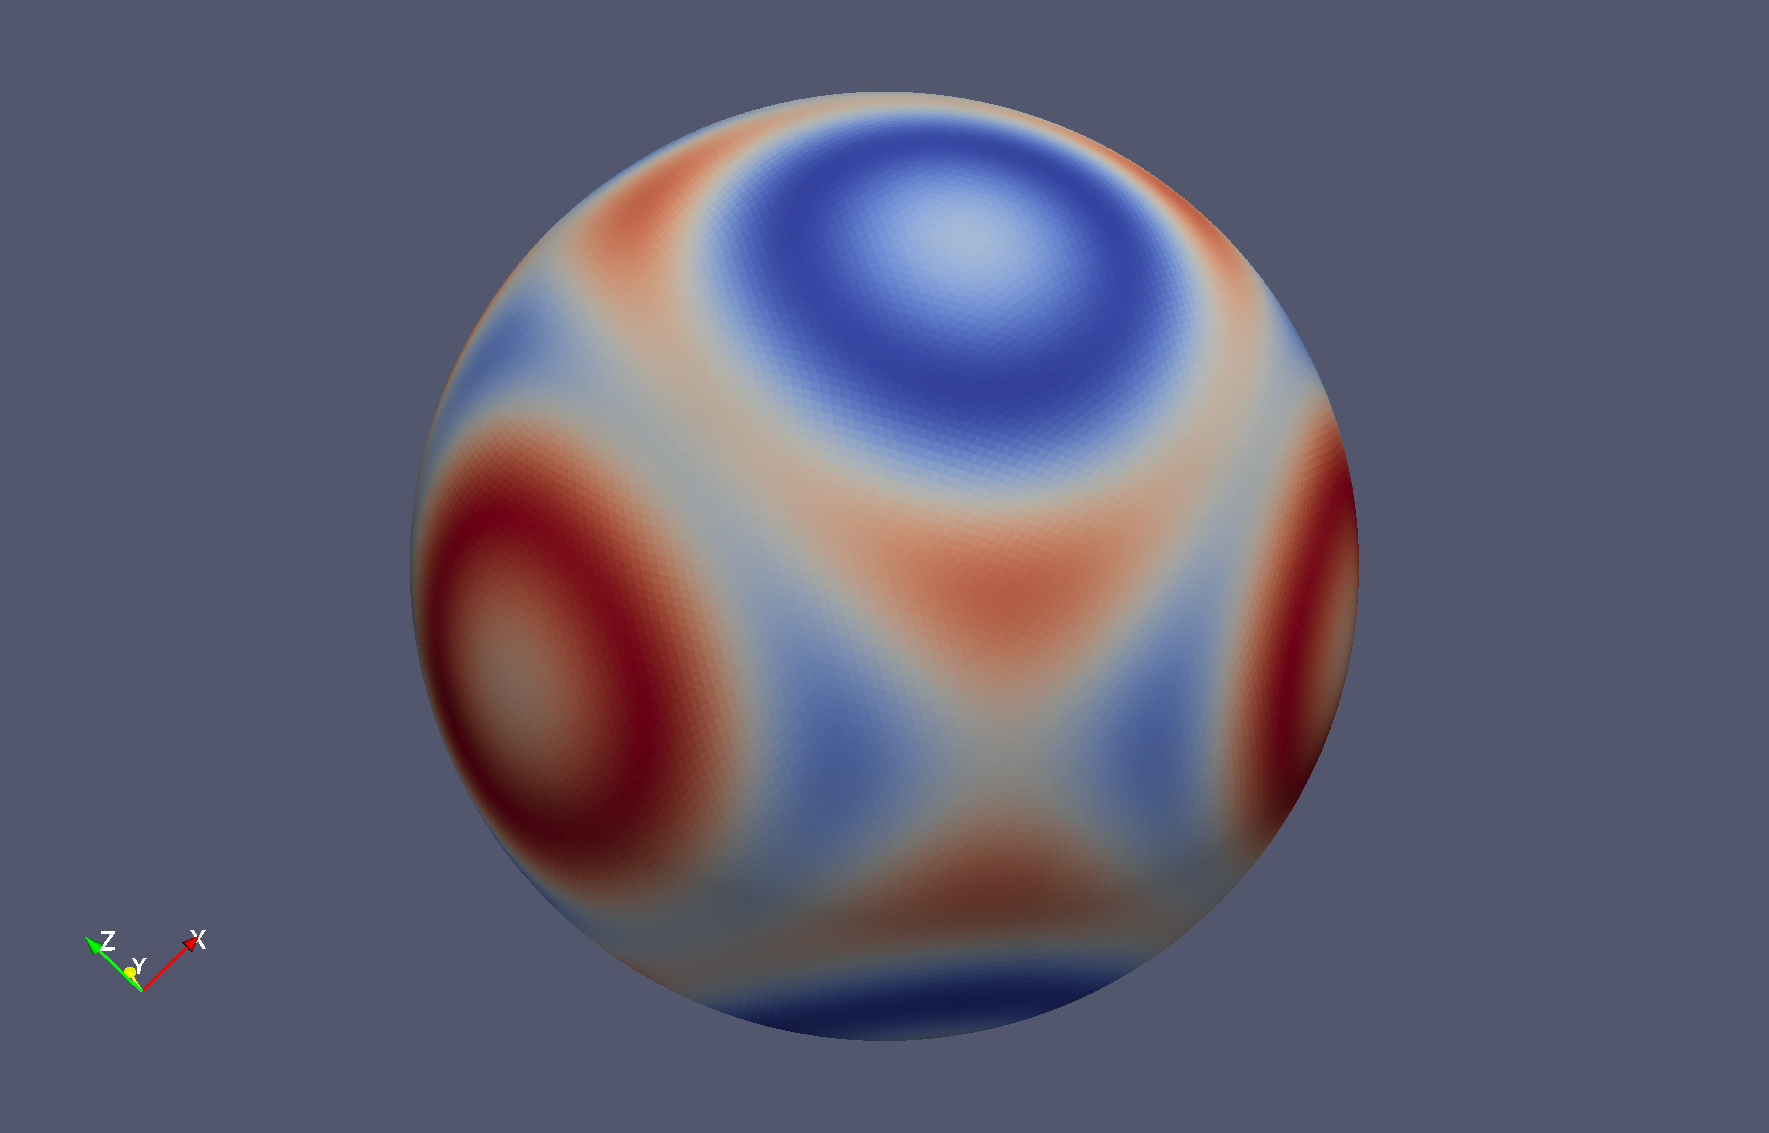
\includegraphics[width=\textwidth]{03-12-PRISM-firedrake-overview.figures/sphere}
\end{center}
\end{frame}


\begin{frame}[label={sec:orgheadline7}]{Express what, not how}
\begin{itemize}
\item User code should make as few decisions about implementation as
possible
\item FE discretisations expressed symbolically using the \emph{Unified Form Language}
\begin{itemize}
\item developed in the FEniCS project (\url{http://www.fenicsproject.org})
\item symbolic representation compiled to a C kernel
\end{itemize}
\item Data to feed to kernel (and interface to solvers) provided by
Firedrake (\url{http://www.firedrakeproject.org})
\item Execution of kernel over entire domain expressed as parallel loop
with access descriptors
\begin{itemize}
\item uses PyOP2 unstructured mesh library (\url{http://github.com/OP2/PyOP2})
\end{itemize}
\end{itemize}
\end{frame}

\begin{frame}[plain,label={sec:orgheadline8}]{Firedrake}
\begin{center}
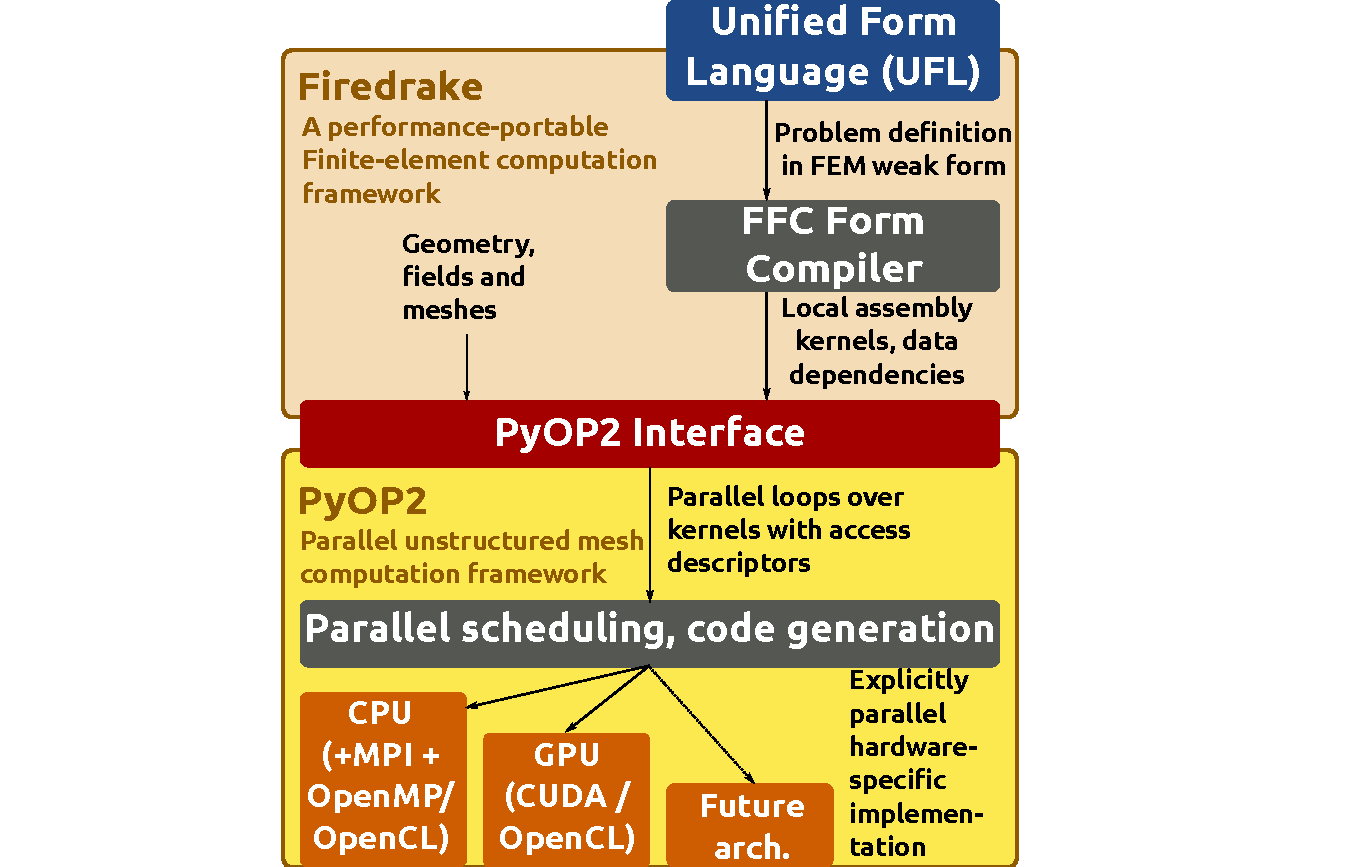
\includegraphics[height=1\textheight]{03-12-PRISM-firedrake-overview.figures/firedrake_toolchain}
\end{center}
\end{frame}

\begin{frame}[label={sec:orgheadline9}]{Firedrake guiding principles}
\begin{itemize}
\item \emph{Everything} is data parallel (user should not care about MPI,
modulo bugs)
\item Objects retain information as long as possible
\begin{itemize}
\item e.g. assembled matrices remember the form they were assembled from
\end{itemize}
\item If someone else has a solution, use it
\begin{itemize}
\item all solves are delegated to PETSc
\item mesh infrastructure too (soon!)
\end{itemize}
\item We do no computation ourselves
\begin{itemize}
\item all iteration over meshes is carried out in PyOP2
\end{itemize}
\end{itemize}
\end{frame}

\begin{frame}[label={sec:orgheadline10}]{Non-FEM kernels}
\begin{itemize}
\item For variational problems, UFL+FFC toolchain generate kernels
automatically
\item You can also write them by hand
\begin{itemize}
\item e.g. for slope limiters
\end{itemize}
\end{itemize}
\end{frame}

\begin{frame}[label={sec:orgheadline11}]{PyOP2 data model}
\begin{itemize}
\item User writes a \emph{local} kernel, operating on \emph{local} data
\item \emph{Maps} are used to describe how \emph{global} data maps to \emph{local} data
\begin{itemize}
\item this comes from mesh topology
\end{itemize}
\item \emph{parallel loop} executes \emph{local} kernel everywhere on mesh (feeding
it the correct global data)
\item access descriptors
\begin{itemize}
\item READ, RW, WRITE, INC, \ldots{}
\item allow reasoning about execution patterns
\end{itemize}
\end{itemize}
\end{frame}

\begin{frame}[fragile,label={sec:orgheadline12}]{Code generation by synthesis at runtime}
 \begin{itemize}
\item \texttt{par\_loop} translated into low-level code (C/Cuda/OpenCL)
\item you promise the execution order doesn't matter
\item we promise to take care of possible data races
\end{itemize}
\end{frame}

\begin{frame}[fragile,label={sec:orgheadline13}]{Why runtime?}
 \begin{itemize}
\item No (complicated) analysis of program is required

\item Access descriptors on parallel loops mean (for example):
\begin{itemize}
\item code generation is only a synthesis problem
\item determination of when halo exchanges need to occur is automatic
(no more \texttt{call halo\_update} sprinkling)
\item colouring for shared memory parallelisation can be computed
automatically
\end{itemize}

\item Lazy/delayed computation, loop fusion, reordering reasonably
straightforward
\end{itemize}
\end{frame}

\section{Exploiting structure}
\label{sec:orgheadline18}

\begin{frame}[label={sec:orgheadline15}]{Extruded meshes}
\begin{itemize}
\item Many application areas have a "short" direction
\begin{itemize}
\item ocean and atmosphere
\item thin shells
\end{itemize}
\item Numerics dictate we should do something different in short
direction
\item Use extruded meshes
\begin{itemize}
\item unstructured in "long" directions, structured in short
\end{itemize}
\end{itemize}
\end{frame}

\begin{frame}[label={sec:orgheadline16}]{A picture of triangles}
\begin{center}
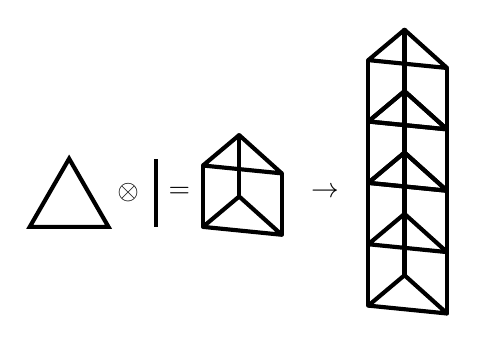
\begin{tikzpicture}[scale=1]
\draw[line width=1.5pt] (0,0) -- (1,0) -- (60:1) -- cycle;
\node at (1.25,0 |- 60:0.5) {$\otimes$};
\draw[line width=1.5pt] (1.6,0) -- (1.6,0 |- 60:1);
\node at (1.9,0 |- 60:0.5) {$=$};

\draw[line width=1.5pt, line join=bevel] (2.2,0) -- +(1, -0.1) -- +(40:0.6) -- cycle;

\draw[line width=1.5pt, line cap=round] (2.2, 0) -- +(0,0 |- 60:0.9);
\draw[line width=1.5pt, line cap=round] (2.2, 0) ++(1, -0.1) -- +(0,0 |- 60:0.9);
\draw[line width=1.5pt, line cap=round] (2.2, 0) ++(40:0.6) -- +(0,0 |- 60:0.9);
\draw[line width=1.5pt, line join=bevel] (2.2,0) ++(0,0 |- 60:0.9) --
+(1, -0.1) -- +(40:0.6) -- cycle;

\node at (3.75, 0 |- 60:0.5) {$\rightarrow$};
% ++(0,0 |- 60:1) -- +(1, -0.25) -- +(40:0.7) -- (2, 0 |- 60:1);

\draw[line width=1.5pt, line join=bevel] (4.3, -1) -- +(1, -0.1) -- +(40:0.6) -- cycle;
\draw[line width=1.5pt, line cap=round] (4.3, -1) -- +(0,0 |- 60:0.9);
\draw[line width=1.5pt, line cap=round] (4.3, -1) ++(1, -0.1) -- +(0,0 |- 60:0.9);
\draw[line width=1.5pt, line cap=round] (4.3, -1) ++(40:0.6) -- +(0,0 |- 60:0.9);
\draw[line width=1.5pt, line join=bevel] (4.3, -1) ++(0,0 |- 60:0.9) -- +(1, -0.1) -- +(40:0.6) -- cycle;

\draw[line width=1.5pt, line cap=round] (4.3, -1) ++(0,0 |- 60:0.9) -- +(0,0 |- 60:0.9);
\draw[line width=1.5pt, line cap=round] (4.3, -1) ++(0,0 |- 60:0.9) ++(1, -0.1) -- +(0,0 |- 60:0.9);
\draw[line width=1.5pt, line cap=round] (4.3, -1) ++(0,0 |- 60:0.9) ++(40:0.6) -- +(0,0 |- 60:0.9);
\draw[line width=1.5pt, line join=bevel] (4.3, -1) ++(0,0 |- 60:0.9) ++(0,0 |- 60:0.9) -- +(1, -0.1) -- +(40:0.6) -- cycle;

\draw[line width=1.5pt, line join=bevel] (4.3, -1) ++(0,0 |- 60:1.8) -- +(1, -0.1) -- +(40:0.6) -- cycle;
\draw[line width=1.5pt, line cap=round] (4.3, -1) ++(0,0 |- 60:1.8) -- +(0,0 |- 60:0.9);
\draw[line width=1.5pt, line cap=round] (4.3, -1) ++(0,0 |- 60:1.8) ++(1, -0.1) -- +(0,0 |- 60:0.9);
\draw[line width=1.5pt, line cap=round] (4.3, -1) ++(0,0 |- 60:1.8) ++(40:0.6) -- +(0,0 |- 60:0.9);
\draw[line width=1.5pt, line join=bevel] (4.3, -1) ++(0,0 |- 60:1.8) ++(0,0 |- 60:0.9) -- +(1, -0.1) -- +(40:0.6) -- cycle;

\draw[line width=1.5pt, line join=bevel] (4.3, -1) ++(0,0 |- 60:2.7) -- +(1, -0.1) -- +(40:0.6) -- cycle;
\draw[line width=1.5pt, line cap=round] (4.3, -1) ++(0,0 |- 60:2.7) -- +(0,0 |- 60:0.9);
\draw[line width=1.5pt, line cap=round] (4.3, -1) ++(0,0 |- 60:2.7) ++(1, -0.1) -- +(0,0 |- 60:0.9);
\draw[line width=1.5pt, line cap=round] (4.3, -1) ++(0,0 |- 60:2.7) ++(40:0.6) -- +(0,0 |- 60:0.9);
\draw[line width=1.5pt, line join=bevel] (4.3, -1) ++(0,0 |- 60:2.7) ++(0,0 |- 60:0.9) -- +(1, -0.1) -- +(40:0.6) -- cycle;
\end{tikzpicture}
\end{center}
\end{frame}

\begin{frame}[fragile,label={sec:orgheadline17}]{Firedrake support}
 \begin{itemize}
\item Tensor product structure available at symbolic level
\end{itemize}
\begin{minted}[frame=none,xleftmargin=1em,xrightmargin=1em,fontsize=\scriptsize,mathescape]{python}
m = Mesh(...)
# 100 cell layers each 0.1 units high
e = ExtrudedMesh(m, layers=100, layer_height=0.1)
U0 = FiniteElement('CG', 'triangle', 1)
U1 = FiniteElement('RT', 'triangle', 1)
V0 = FiniteElement('CG', 'interval', 3)
V1 = FiniteElement('DG', 'interval', 2)
# $W_1 = (U_1\otimes{}V_0)\oplus{}(U_0\otimes{}V_1)\subset{}H_\mathrm{curl}$
W1 = HCurl(OuterProductElement(U1, V0)) + \
     HCurl(OuterProductElement(U0, V1))
...
\end{minted}
\begin{itemize}
\item Code generation currently throws this away (tensor products expanded
too early)
\end{itemize}
\end{frame}

\section{Mesh numbering}
\label{sec:orgheadline22}
\begin{frame}[fragile,label={sec:orgheadline19}]{A bandwidth bound test}
 \begin{itemize}
\item Walk over mesh, read from vertices and cells, sum into global
\end{itemize}
\begin{minted}[frame=none,xleftmargin=1em,xrightmargin=1em,fontsize=\scriptsize,mathescape]{c}
void kernel(double *a, double *x[], double *y[]) {
    const double area = fabs(x[0][0]*(x[2][1]-x[4][1])
                             + x[2][0]*(x[4][1]-x[0][1])
                             + x[4][0]*(x[0][1]-x[2][1]));
    *a += area * 0.5 * y[0][0];
}
\end{minted}
\begin{itemize}
\item Can we sustain an appreciable fraction of memory bandwidth?
\end{itemize}
\end{frame}

\begin{frame}[label={sec:orgheadline20}]{Effect of good base numbering}
\begin{itemize}
\item Being completely unstructured hurts a lot
\item Compare default (mesh generator) numbering with renumbered mesh
using 2D space filling curve
\end{itemize}
\begin{center}
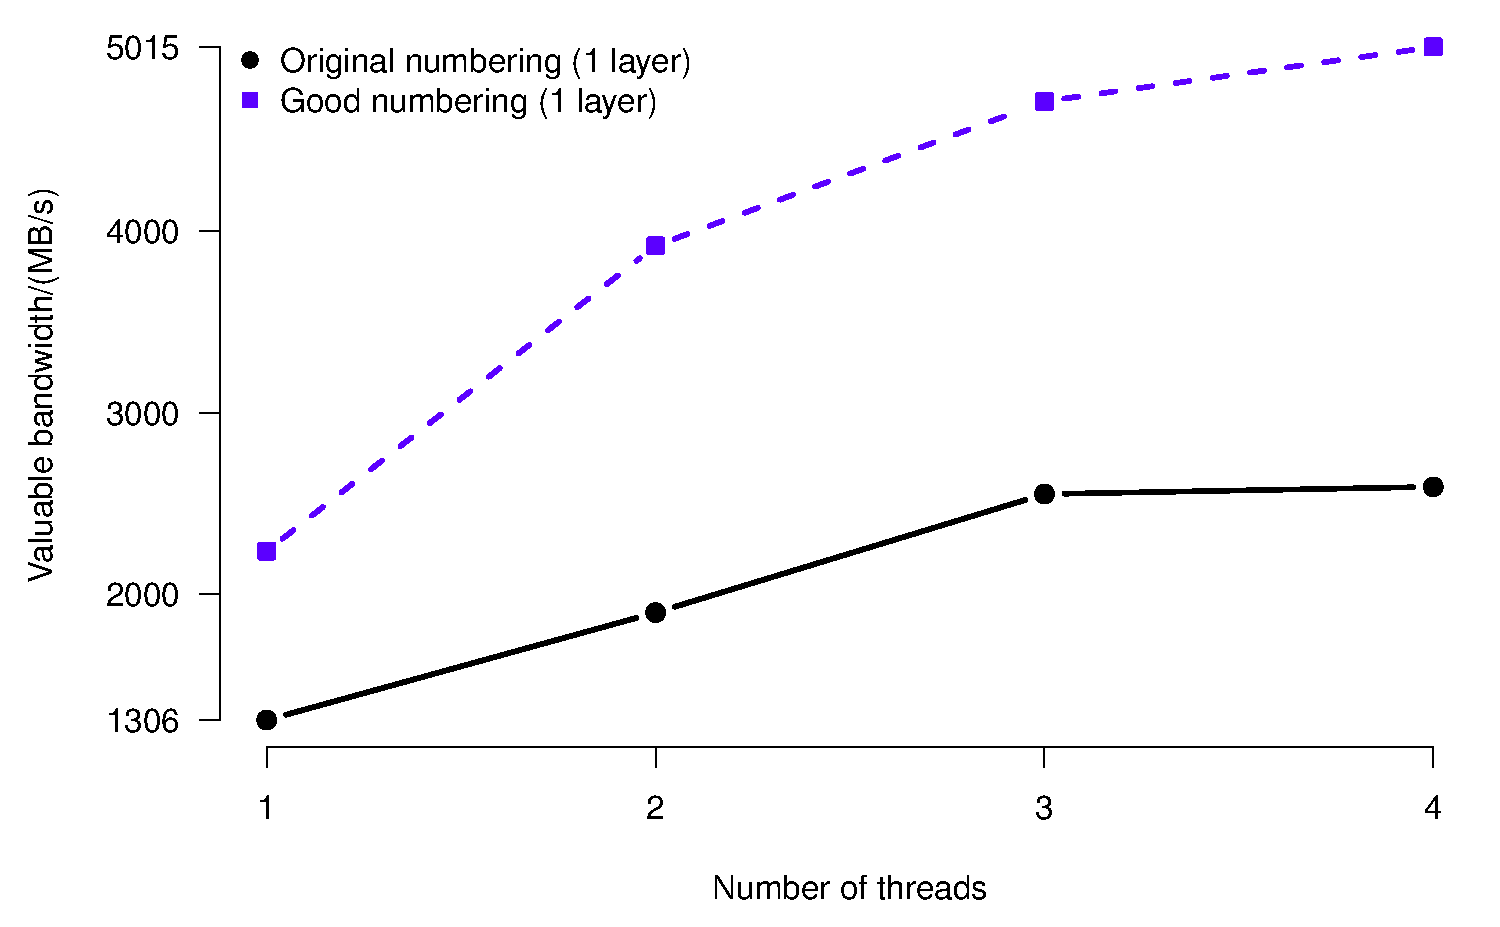
\includegraphics[height=0.8\textheight]{03-12-PRISM-firedrake-overview.figures/bad-numbering}
\end{center}
\end{frame}

\begin{frame}[label={sec:orgheadline21}]{More threads and layers}
\begin{itemize}
\item With layers, achieve 82\% STREAM bandwidth
\end{itemize}
\begin{center}
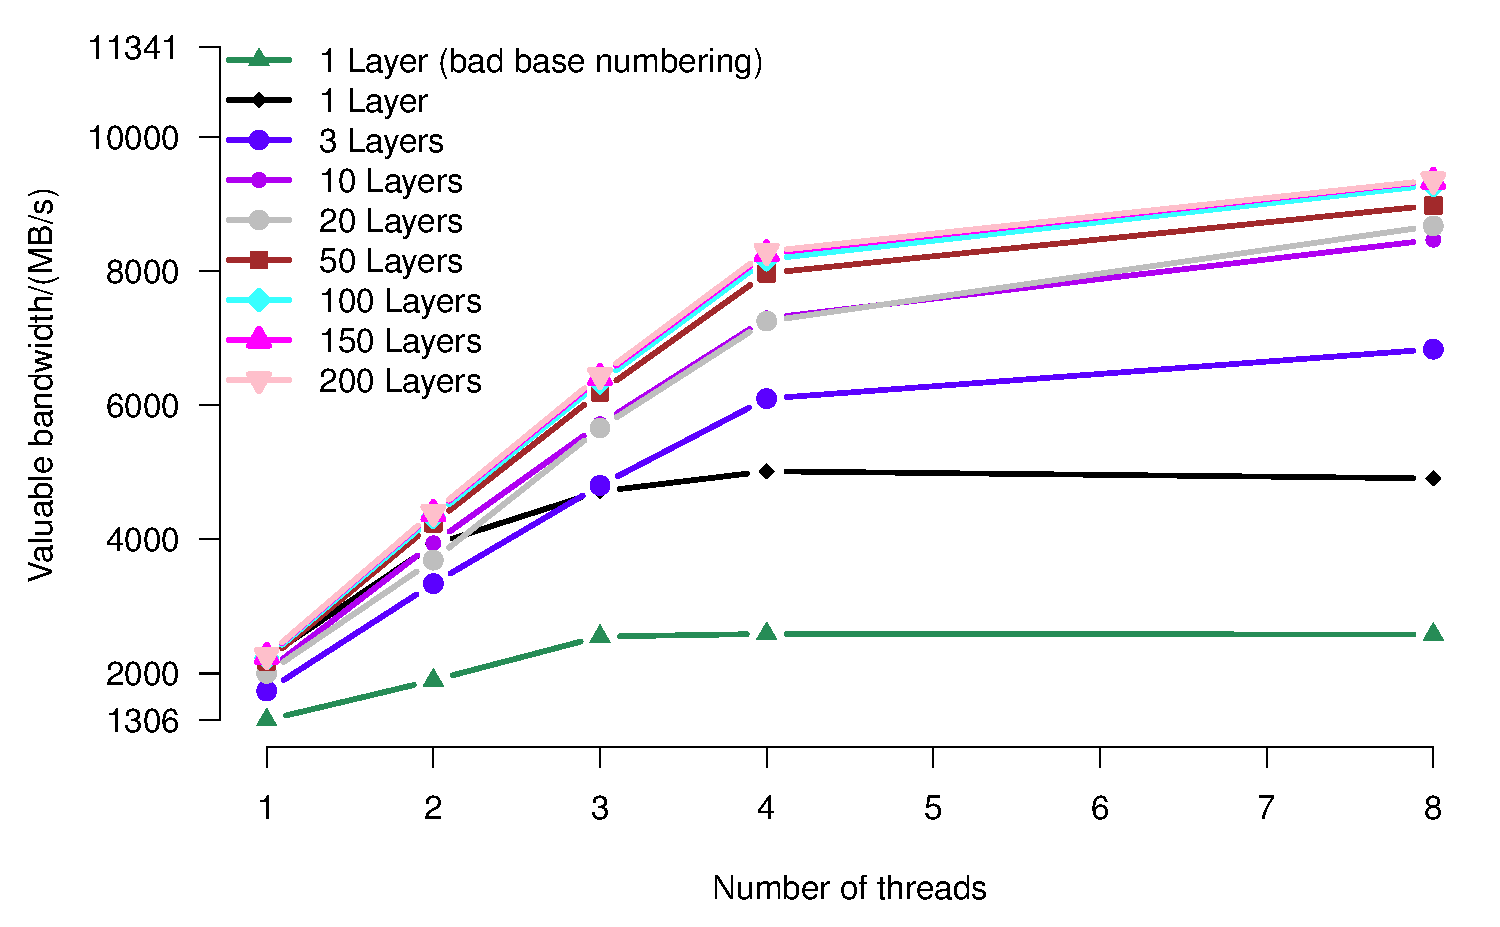
\includegraphics[height=0.8\textheight]{03-12-PRISM-firedrake-overview.figures/valuable-bandwidth-by-thread}
\end{center}
\end{frame}


\section{Solving PDEs}
\label{sec:orgheadline25}

\begin{frame}[fragile,label={sec:orgheadline23}]{Coupled systems}
 \begin{itemize}
\item Block structure in the equations, mirrored in Firedrake objects
\end{itemize}
\begin{minted}[frame=none,xleftmargin=1em,xrightmargin=1em,fontsize=\scriptsize,mathescape]{python}
# Poisson example from before
# $a(\sigma,u;\tau,v)=\int_{\Omega}\sigma\cdot\tau+\nabla\cdot\sigma{}v+\nabla\cdot\tau{}u\mathrm{d}x$
a = (inner(sigma, tau) + div(sigma)*v + div(tau)*u)*dx
A = assemble(a)
# $\sigma\cdot\tau$ piece
A.M[0, 0]
# $\nabla\cdot{}\sigma{}v$ piece
A.M[1, 0]
# $\nabla\cdot{}\tau{}u$ piece
A.M[0, 1]
# $uv$ piece (just zero)
A.M[1, 1]
\end{minted}
\begin{itemize}
\item We can use PETSc's "physics-based" preconditioners
\begin{itemize}
\item Schur complements and so forth
\end{itemize}
\end{itemize}
\end{frame}

\begin{frame}[fragile,label={sec:orgheadline24}]{Nonlinear PDEs}
 \begin{itemize}
\item You provide the residual, we (Martin!) differentiate symbolically to get the
Jacobian
\begin{itemize}
\item Hooked into PETSc \texttt{SNES}
\item various Newton-like nonlinear solves
\end{itemize}
\end{itemize}

\begin{minted}[frame=none,xleftmargin=1em,xrightmargin=1em,fontsize=\scriptsize,mathescape]{python}
...
# $\int_\Omega\frac{u^{n+1}-u^n}{dt}\cdot{}v+(u^{n+1}\cdot\nabla{}u^{n+1})\cdot{}v+\nu\nabla{}u^{n+1}\cdot\nabla{}v\;\mathrm{d}x = 0$
F = (inner((u - u_)/timestep, v) +
     inner(u, dot(grad(u), v)) +
     nu*inner(grad(u), grad(v)))*dx
...
while (t <= end):
    # $J=\mathrm{d}F$ computed symbolically
    # F = derivative(F, u)
    solve(F == 0, u, solver_parameters={...})
    u_.assign(u)
    t += dt
\end{minted}
\end{frame}
\section{Roadmap}
\label{sec:orgheadline28}

\begin{frame}[label={sec:orgheadline26}]{What's coming}
\begin{itemize}
\item DMPlex (PETSc) mesh infrastructure [imminently]
\item Hierarchy of function spaces (for multigrid)
\item Non-affine elements (symbolically)
\item Less stupid tensor product kernels
\item Unstructured quads
\item Matrix free
\item More performance
\item GPU feature parity?
\end{itemize}
\end{frame}

\begin{frame}[label={sec:orgheadline27}]{Links}
\begin{itemize}
\item \url{http://www.firedrakeproject.org}
\item \url{http://op2.github.com/PyOP2}
\item firedrake@imperial.ac.uk
\item \#firedrake on irc.freenode.net
\end{itemize}
\end{frame}
\end{document}
